\documentclass[aspectratio=169,11pt]{beamer}

\usepackage[utf8]{inputenc}
\usepackage[T1]{fontenc}
\usepackage{amsmath,amssymb,bm}
\usepackage{tikz}
\usepackage{pgfplots}
\pgfplotsset{compat=1.18}
\usetikzlibrary{positioning,arrows.meta,calc,backgrounds}
\usepackage{xcolor}
\usepackage{listings}
\usepackage{microtype}
\usepackage{booktabs}
\usepackage{hyperref}
\hypersetup{colorlinks=true,urlcolor=accentblue,linkcolor=.}

% ── Paleta ────────────────────────────────────────────────────────────────────
\definecolor{darkbg}{HTML}{0D2137}
\definecolor{midbg}{HTML}{1A3550}
\definecolor{lightbg}{HTML}{F4F7FA}
\definecolor{accentblue}{HTML}{4A9CC7}
\definecolor{accentteal}{HTML}{2AB0A0}
\definecolor{accentgold}{HTML}{D4A843}
\definecolor{accentred}{HTML}{C0392B}
\definecolor{accentpurple}{HTML}{7B68EE}
\definecolor{codebg}{HTML}{1E2B3C}
\definecolor{codegreen}{HTML}{50C878}
\definecolor{codeyellow}{HTML}{FFD700}
\definecolor{textdark}{HTML}{1A2B3C}
\definecolor{textmid}{HTML}{4A5568}
\definecolor{boxblue}{HTML}{EBF4FA}
\definecolor{boxteal}{HTML}{E6F5F3}
\definecolor{boxgold}{HTML}{FDF6E3}
\definecolor{boxred}{HTML}{FDECEA}

% ── Tema ──────────────────────────────────────────────────────────────────────
\usetheme{default}
\usecolortheme{default}
\usefonttheme{professionalfonts}
\setbeamertemplate{navigation symbols}{}
\usepackage{helvet}
\renewcommand{\familydefault}{\sfdefault}

\setbeamercolor{normal text}{fg=textdark,bg=lightbg}
\setbeamercolor{frametitle}{fg=darkbg,bg=lightbg}
\setbeamercolor{block title}{fg=white,bg=accentblue}
\setbeamercolor{block body}{fg=textdark,bg=boxblue}
\setbeamercolor{block title alerted}{fg=white,bg=accentred}
\setbeamercolor{block body alerted}{fg=textdark,bg=boxred}
\setbeamercolor{block title example}{fg=white,bg=accentteal}
\setbeamercolor{block body example}{fg=textdark,bg=boxteal}
\setbeamercolor{footline}{fg=textmid}

\setbeamertemplate{frametitle}{%
  \vspace{0.3cm}%
  {\color{darkbg}\textbf{\large\insertframetitle}}%
  \ifx\insertframesubtitle\@empty\else%
    \\[0.03cm]{\color{textmid}\footnotesize\insertframesubtitle}\fi%
  \vspace{0.08cm}%
  {\color{accentblue}\hrule height 1.1pt}%
  \vspace{0.04cm}}

\setbeamertemplate{footline}{%
  \begin{beamercolorbox}[wd=\paperwidth,ht=0.35cm,dp=0.15cm]{footline}%
    \hspace{0.4cm}{\tiny\color{textmid}Programaci\'on Cient\'ifica 2026-1 $\cdot$ UNAL}%
    \hfill{\tiny\color{textmid}\insertframenumber/\inserttotalframenumber\hspace{0.4cm}}%
  \end{beamercolorbox}}

\setbeamertemplate{itemize item}{\color{accentblue}\textbf{--}}
\setbeamertemplate{itemize subitem}{\color{accentteal}\small$\circ$}
\setlength{\leftmargini}{1.1em}

% ── Listings: estilo terminal oscuro ──────────────────────────────────────────
\lstset{
  language=Python,
  backgroundcolor=\color{codebg},
  basicstyle=\ttfamily\footnotesize\color{white},
  keywordstyle=\color{accentblue}\bfseries,
  stringstyle=\color{codegreen},
  commentstyle=\color{textmid}\itshape,
  numberstyle=\tiny\color{textmid},
  identifierstyle=\color{white},
  emphstyle=\color{codeyellow}\bfseries,
  emph={import,from,as,True,False,None},
  frame=none,
  xleftmargin=6pt,
  xrightmargin=6pt,
  aboveskip=4pt,
  belowskip=2pt,
  showstringspaces=false,
  breaklines=true,
  tabsize=2,
  literate={á}{{\'a}}1 {é}{{\'e}}1 {í}{{\'i}}1 {ó}{{\'o}}1 {ú}{{\'u}}1
           {ñ}{{\~n}}1 {Á}{{\'A}}1 {É}{{\'E}}1 {Í}{{\'I}}1 {Ó}{{\'O}}1
}

% ── Macros ────────────────────────────────────────────────────────────────────
\newcommand{\R}{\mathbb{R}}
\newcommand{\vc}{\mathbf{c}}
\newcommand{\vy}{\mathbf{y}}
\newcommand{\norm}[1]{\left\|#1\right\|}

\newcommand{\fmbox}[2][accentblue]{%
  \begin{center}\tikz\node[draw=#1,fill=#1!8,rounded corners=3pt,
    inner sep=7pt,line width=1.1pt]{$\displaystyle #2$};\end{center}}

\newcommand{\keybox}[2]{%
  \begin{center}\begin{tikzpicture}
    \node[draw=accentgold,fill=boxgold,rounded corners=3pt,
          inner sep=7pt,line width=1.1pt,text width=0.87\textwidth]{%
      {\color{accentgold}\textbf{#1}}\enspace #2};
  \end{tikzpicture}\end{center}}

\newcommand{\sectionslide}[3]{%
  {\setbeamercolor{background canvas}{bg=midbg}
  \begin{frame}[plain]
    \begin{tikzpicture}[remember picture,overlay]
      \fill[darkbg!80,opacity=0.6](current page.north east)++(-1,-1)circle(3.5cm);
      \fill[accentteal,opacity=0.15](current page.south west)++(2,1)circle(2.5cm);
      \fill[darkbg,opacity=0.4](current page.south east)++(-3,2)circle(1.8cm);
      \node[anchor=west] at ([xshift=1.2cm,yshift=0.9cm]current page.west)
        {\color{accentblue}\fontsize{17}{20}\selectfont\textbf{#1}};
      \node[anchor=west] at ([xshift=1.2cm,yshift=0.1cm]current page.west)
        {\color{white}\fontsize{30}{34}\selectfont\textbf{#2}};
      \draw[accentblue,line width=2pt]
        ([xshift=1.2cm,yshift=-0.55cm]current page.west)--
        ([xshift=6cm,yshift=-0.55cm]current page.west);
      \node[anchor=west,text width=10cm] at ([xshift=1.2cm,yshift=-1.2cm]current page.west)
        {\color{white!70!accentblue}\large #3};
    \end{tikzpicture}
  \end{frame}}}

% Slide de pausa activa
\newcommand{\pausaslide}[3]{%
  {\setbeamercolor{background canvas}{bg=darkbg}
  \begin{frame}[plain]
    \begin{tikzpicture}[remember picture,overlay]
      \fill[accentgold,opacity=0.08](current page.center)circle(5cm);
      \node[anchor=center,yshift=1.2cm] at (current page.center)
        {\color{accentgold}\fontsize{14}{16}\selectfont\textbf{$\bigstar$ Pausa activa #1}};
      \node[anchor=center,text width=12cm,align=center] at (current page.center)
        {\color{white}\fontsize{14}{18}\selectfont #2};
      \node[anchor=center,yshift=-1.8cm,text width=11cm,align=center] at (current page.center)
        {\color{white!60!accentblue}\small #3};
    \end{tikzpicture}
  \end{frame}}}

% ══════════════════════════════════════════════════════════════════════════════
\begin{document}
\setbeamercolor{background canvas}{bg=lightbg}

% ── PORTADA ───────────────────────────────────────────────────────────────────
{\setbeamercolor{background canvas}{bg=darkbg}
\begin{frame}[plain]
  \begin{tikzpicture}[remember picture,overlay]
    \fill[accentblue,opacity=0.10](current page.north east)++(-2,-2)circle(4cm);
    \fill[accentteal,opacity=0.08](current page.south west)++(3,2)circle(3cm);
    \fill[midbg,opacity=0.5](current page.south east)++(-4,3)circle(2.2cm);
    \node[anchor=west] at ([xshift=1.2cm,yshift=2.3cm]current page.west)
      {\color{white!60!accentblue}\small Universidad Nacional de Colombia, Medellín $\cdot$ Programaci\'on Cient\'ifica 2026-1};
    \draw[accentblue,line width=0.8pt]
      ([xshift=1.2cm,yshift=1.9cm]current page.west)--
      ([xshift=14cm,yshift=1.9cm]current page.west);
    \node[anchor=west,text width=14cm] at ([xshift=1.2cm,yshift=0.7cm]current page.west)
      {\color{white}\fontsize{24}{30}\selectfont\textbf{Aproximaci\'on de "curvas"}};
    \node[anchor=west,text width=14cm] at ([xshift=1.2cm,yshift=-0.4cm]current page.west)
      {\color{accentteal}\large Interpolaci\'on $\to$ Splines $\to$ B\'ezier $\to$ B-splines $\to$ LS $\to$ PCA};
    \node[anchor=west] at ([xshift=1.2cm,yshift=-1.3cm]current page.west)
      {\color{white!50!accentblue}\small Manuela Bastidas Olivares};
  \end{tikzpicture}
\end{frame}}

% ── PREGUNTA CONDUCTORA ───────────────────────────────────────────────────────
\begin{frame}{Una sola pregunta conduce toda la clase}
  \vspace{0.1cm}
  \begin{center}
  \tikz\node[draw=accentblue,fill=boxblue,rounded corners=5pt,
             inner sep=14pt,line width=1.5pt,text width=11cm,align=center]{%
    {\color{accentblue}\Large\textbf{?`C\'omo representar datos con funciones suaves?}}\\[8pt]
    {\color{textmid} \underline{Todos} los m\'etodos son: $\displaystyle f(t) = \sum_{i} c_i\,\phi_i(t)$}\\[4pt]
    {\color{textmid}\small La diferencia est\'a en la \textbf{elecci\'on de la base} $\{\phi_i\}$}};
  \end{center}
  \vspace{0.2cm}
  \begin{center}
  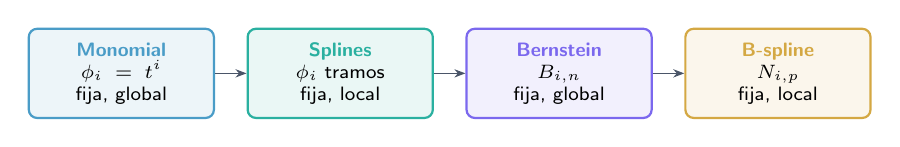
\begin{tikzpicture}[node distance=0.35cm and 0.4cm,
      arr/.style={-{Stealth[length=4pt]},textmid,thin},
      arr/.style={-{Stealth[length=4pt]},textmid,thin}]
    \node[draw=accentblue,fill=accentblue!10,rounded corners=3pt,inner sep=5pt,
          text width=2.0cm,align=center,font=\scriptsize,line width=0.8pt](a1)
      {\textbf{\color{accentblue}Monomial}\\$\phi_i=t^i$\\fija, global};
    \node[draw=accentteal,fill=accentteal!10,rounded corners=3pt,inner sep=5pt,
          text width=2.0cm,align=center,font=\scriptsize,line width=0.8pt,right=of a1](a2)
      {\textbf{\color{accentteal}Splines}\\$\phi_i$ tramos\\fija, local};
    \node[draw=accentpurple,fill=accentpurple!10,rounded corners=3pt,inner sep=5pt,
          text width=2.0cm,align=center,font=\scriptsize,line width=0.8pt,right=of a2](a3)
      {\textbf{\color{accentpurple}Bernstein}\\$B_{i,n}$\\fija, global};
    \node[draw=accentgold,fill=accentgold!10,rounded corners=3pt,inner sep=5pt,
          text width=2.0cm,align=center,font=\scriptsize,line width=0.8pt,right=of a3](a4)
      {\textbf{\color{accentgold}B-spline}\\$N_{i,p}$\\fija, local};
    \draw[-{Stealth[length=4pt]},textmid,thin](a1)--(a2);
    \draw[-{Stealth[length=4pt]},textmid,thin](a2)--(a3);
    \draw[-{Stealth[length=4pt]},textmid,thin](a3)--(a4);
  \end{tikzpicture}
  \end{center}
\end{frame}

% ══════════════════════════════════════════════════════════════════════════════
\sectionslide{1}{Interpolaci\'on}{Retomemos: bases, sistemas y el problema de Runge}

\begin{frame}[fragile]{Todo es una base: monomial, Lagrange, Hermite}
  \fmbox[accentblue]{A\,\mathbf{c} = \mathbf{y}, \qquad A_{ki} = \phi_i(t_k), \qquad \text{sistema cuadrado } (n{+}1)\times(n{+}1)}
  \vspace{0.1cm}
  \begin{columns}[T]
    \column{0.31\textwidth}
      \begin{block}{Monomial \enspace $\phi_i = t^i$}
        \vspace{2pt}
        $A$ = Vandermonde\\
        {\footnotesize Mal condicionada para $n$ grande}\\[4pt]
        \begin{lstlisting}
# numpy lo hace directo
c = np.polyfit(t,y,n)
p = np.polyval(c,t_n)
        \end{lstlisting}
      \end{block}

    \column{0.31\textwidth}
      \begin{exampleblock}{Lagrange \enspace $\phi_i(t_j)=\delta_{ij}$}
        \vspace{2pt}
        $A = I$ \enspace trivial: $c_i = y_i$\\
        {\footnotesize Oscila en extremos (Runge)}\\[4pt]
        \begin{lstlisting}
from scipy.interpolate \
  import lagrange
p = lagrange(t,y)
y_new = p(t_n)
        \end{lstlisting}
      \end{exampleblock}

    \column{0.31\textwidth}
      \begin{alertblock}{Hermite \enspace valores+derivadas}
        \vspace{2pt}
        $2(n{+}1)$ condiciones\\
        {\footnotesize Controla tangentes}\\[3pt]
        \begin{lstlisting}
from scipy.interpolate \
import CubicHermiteSpline
        \end{lstlisting}
      \end{alertblock}
  \end{columns}
\end{frame}

\begin{frame}{El problema de Runge: por qu\'e la base importa}
	\begin{columns}[T]
		\column{0.50\textwidth}
		\begin{center}
			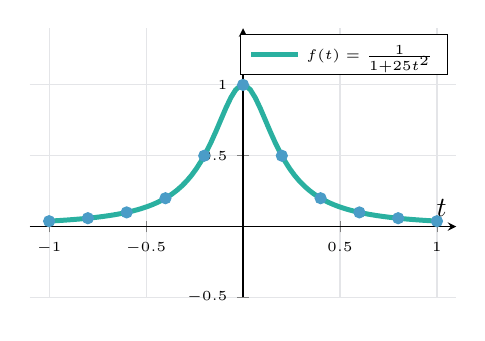
\begin{tikzpicture}
				\begin{axis}[width=7cm,height=5cm,
					domain=-1:1,samples=80,
					xmin=-1.1,xmax=1.1,ymin=-0.5,ymax=1.4,
					axis lines=center,xlabel={$t$},
					tick label style={font=\tiny},
					grid=both,grid style={color=textmid!15},
					legend style={font=\tiny,at={(0.98,0.98)},anchor=north east}]
					\addplot[accentteal,line width=1.8pt]{1/(1+25*x^2)};
					\addlegendentry{$f(t)=\frac{1}{1+25t^2}$}
					%\addplot[accentred,dashed,line width=1.5pt]
					%{1/(1+25*x^2)+0.35*x^2*(x^2-0.16)*(x^2-0.64)*(x^2-1)};
					%\addlegendentry{Lagrange $n=10$}
					\addplot[only marks,mark=*,mark size=2pt,accentblue]
					coordinates{(-1,.038)(-.8,.059)(-.6,.1)(-.4,.2)(-.2,.5)
						(0,1)(.2,.5)(.4,.2)(.6,.1)(.8,.059)(1,.038)};
				\end{axis}
			\end{tikzpicture}
		\end{center}
		
		\column{0.46\textwidth}
		\vspace{0.3cm}
		La base monomial/Lagrange es \textbf{global}: cada $\phi_i$ influye en todo $[{-}1,1]$.
		
		\vspace{0.3cm}
		\begin{alertblock}{Runge}
			Grado $n$ alto + nodos equiespaciados = oscilaciones explosivas en los bordes.
		\end{alertblock}
		
		\vspace{0.2cm}
		\begin{exampleblock}{La soluci\'on}
			Bases con \textbf{soporte local}.\\
			La oscilaci\'on no se propaga
		\end{exampleblock}
	\end{columns}
\end{frame}

\begin{frame}[fragile]{Splines c\'ubicos: base local por tramos}
  \begin{columns}[T]
    \column{0.50\textwidth}
      En cada $[t_k,t_{k+1}]$: $S_k(t) = a_k+b_k h+c_k h^2+d_k h^3$, $h=t-t_k$.

      Condiciones: $S$, $S'$, $S''$ continuas en nodos.

      \fmbox[accentteal]{A\,\mathbf{c} = \mathbf{y}, \quad A \text{ tridiagonal}}

      \begin{lstlisting}
from scipy.interpolate \
import CubicSpline
cs = CubicSpline(t, y)
# base local automatica
y_new = cs(t_new)
y_der = cs(t_new, 1) # S'
      \end{lstlisting}

    \column{0.46\textwidth}
      \begin{center}
      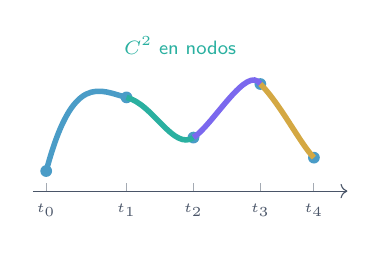
\begin{tikzpicture}[scale=0.85]
        \draw[->,thin,textmid](-0.2,0)--(4.5,0);
        \foreach \x/\y in {0/0.3, 1.2/1.4, 2.2/0.8, 3.2/1.6, 4.0/0.5}{
          \fill[accentblue](\x,\y)circle(2.5pt);}
        \draw[accentblue,line width=2pt]
          (0,0.3)..controls(0.4,1.8)and(0.8,1.5)..(1.2,1.4);
        \draw[accentteal,line width=2pt]
          (1.2,1.4)..controls(1.6,1.3)and(1.9,0.6)..(2.2,0.8);
        \draw[accentpurple,line width=2pt]
          (2.2,0.8)..controls(2.5,1.0)and(3.0,1.9)..(3.2,1.6);
        \draw[accentgold,line width=2pt]
          (3.2,1.6)..controls(3.5,1.3)and(3.8,0.7)..(4.0,0.5);
        \foreach \x/\lbl in {0/t_0,1.2/t_1,2.2/t_2,3.2/t_3,4.0/t_4}{
          \draw[textmid!50,thin,dashed](\x,0)--(\x,0.15);
          \node[below,font=\tiny,color=textmid]at(\x,-0.05){$\lbl$};}
        \node[font=\scriptsize,color=accentteal,above]at(2.0,1.9){$C^2$ en nodos};
      \end{tikzpicture}
      \end{center}

      \vspace{0.2cm}
      \keybox{}{La base son las \textbf{hat functions} c\'ubicas --- soporte local}
  \end{columns}
\end{frame}



% ══════════════════════════════════════════════════════════════════════════════
\sectionslide{2}{B\'ezier y B-splines}{La base como herramienta de dise\~no}

\begin{frame}[fragile]{Base de Bernstein: bella pero global}
  \begin{columns}[T]
    \column{0.48\textwidth}
      \fmbox[accentpurple]{B_{i,n}(t)=\binom{n}{i}t^i(1-t)^{n-i}, \quad \phi_i = B_{i,n}}

      La curva de B\'ezier es:
      \fmbox[accentblue]{\mathbf{C}(t)=\sum_{i=0}^{n}B_{i,n}(t)\,\mathbf{P}_i}

    \column{0.48\textwidth}
      \begin{center}
      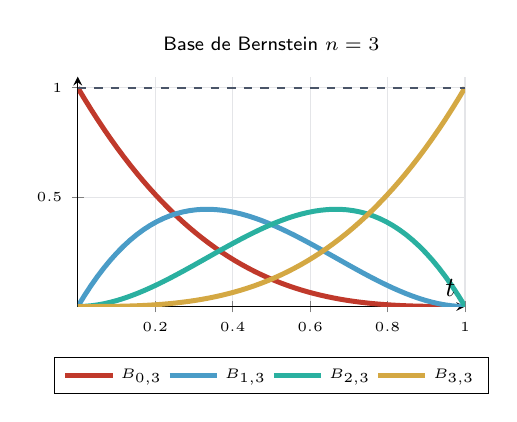
\begin{tikzpicture}
        \begin{axis}[width=6.5cm,height=4.5cm,
          domain=0:1,samples=60,
          xmin=0,xmax=1,ymin=0,ymax=1.05,
          axis lines=center,xlabel={$t$},
          tick label style={font=\tiny},
          grid=both,grid style={color=textmid!15},
          legend style={font=\tiny,at={(0.5,-0.22)},anchor=north,legend columns=4},
          title={\scriptsize Base de Bernstein $n=3$}]
          \addplot[accentred,line width=1.8pt]{(1-x)^3};
          \addlegendentry{$B_{0,3}$}
          \addplot[accentblue,line width=1.8pt]{3*x*(1-x)^2};
          \addlegendentry{$B_{1,3}$}
          \addplot[accentteal,line width=1.8pt]{3*x^2*(1-x)};
          \addlegendentry{$B_{2,3}$}
          \addplot[accentgold,line width=1.8pt]{x^3};
          \addlegendentry{$B_{3,3}$}
          \addplot[textmid,dashed,line width=0.8pt]{1};
        \end{axis}
      \end{tikzpicture}
      \end{center}
      \vspace{0.1cm}
      \begin{center}
      \tikz\node[draw=accentred,fill=boxred,rounded corners=3pt,
                 inner sep=6pt,line width=1pt,text width=5.5cm,align=center,font=\small]{%
        Mover $\mathbf{P}_i$ \textbf{mueve toda la curva}\\porque $B_{i,n}$ es no nula en $[0,1]$};
      \end{center}
  \end{columns}
\end{frame}

\begin{frame}[fragile]{Base de Bernstein: bella pero global}
	\begin{columns}[T]
		\column{0.48\textwidth}
		
		\begin{itemize}
			\item $\sum_i B_{i,n}(t)=1$ (partici\'on)
			\item $B_{i,n}\ge0$ (no negativa)
			\item $\mathbf{C}(0)=\mathbf{P}_0$, $\mathbf{C}(1)=\mathbf{P}_n$
			\item Soporte $[0,1]$ completo 
		\end{itemize}
		
		\begin{lstlisting}
			from scipy.special import comb
			def bernstein(i, n, t):
			return comb(n,i)*t**i*(1-t)**(n-i)
			# curva: suma ponderada
			C = sum(bernstein(i,n,t)*P[i]
			for i in range(n+1))
		\end{lstlisting}
		
		\column{0.48\textwidth}
		\begin{center}
			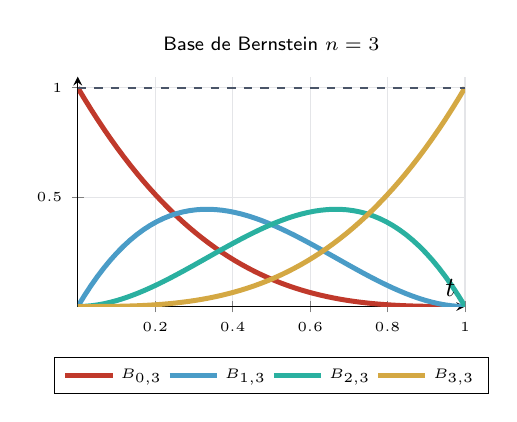
\begin{tikzpicture}
				\begin{axis}[width=6.5cm,height=4.5cm,
					domain=0:1,samples=60,
					xmin=0,xmax=1,ymin=0,ymax=1.05,
					axis lines=center,xlabel={$t$},
					tick label style={font=\tiny},
					grid=both,grid style={color=textmid!15},
					legend style={font=\tiny,at={(0.5,-0.22)},anchor=north,legend columns=4},
					title={\scriptsize Base de Bernstein $n=3$}]
					\addplot[accentred,line width=1.8pt]{(1-x)^3};
					\addlegendentry{$B_{0,3}$}
					\addplot[accentblue,line width=1.8pt]{3*x*(1-x)^2};
					\addlegendentry{$B_{1,3}$}
					\addplot[accentteal,line width=1.8pt]{3*x^2*(1-x)};
					\addlegendentry{$B_{2,3}$}
					\addplot[accentgold,line width=1.8pt]{x^3};
					\addlegendentry{$B_{3,3}$}
					\addplot[textmid,dashed,line width=0.8pt]{1};
				\end{axis}
			\end{tikzpicture}
		\end{center}
		\vspace{0.1cm}
		\begin{center}
			\tikz\node[draw=accentred,fill=boxred,rounded corners=3pt,
			inner sep=6pt,line width=1pt,text width=5.5cm,align=center,font=\small]{%
				Mover $\mathbf{P}_i$ \textbf{mueve toda la curva}\\porque $B_{i,n}$ es no nula en $[0,1]$};
		\end{center}
	\end{columns}
\end{frame}


\begin{frame}[fragile]{Comparaci\'on directa de bases}
  \begin{center}
  \renewcommand{\arraystretch}{1.3}
  \begin{tabular}{lllll}
    \toprule
    \textbf{Base} & \textbf{Soporte} & \textbf{Sistema} & \textbf{Interpola} & \textbf{C\'odigo} \\
    \midrule
    Monomial $t^i$ & global & Vandermonde & s\'i & \texttt{np.polyfit} \\
    Lagrange & global & $A=I$ & s\'i & \texttt{lagrange(t,y)} \\
    Spline c\'ubico & local & tridiagonal & s\'i & \texttt{CubicSpline} \\
    Bernstein $B_{i,n}$ & \textcolor{accentteal}{global} & no-interpola & s\'i extremos & manual \\
    B-spline $N_{i,p}$ & \textcolor{accentred}{local} & no-interpola & s\'i extremos & \texttt{BSpline} \\
    \bottomrule
  \end{tabular}
  \end{center}

  \vspace{0.1cm}
  \keybox{}{Todos son $f(t)=\sum c_i\phi_i(t)$. La base define la estructura de $A$ y las propiedades de $f$.}
\end{frame}


% ══════════════════════════════════════════════════════════════════════════════
\sectionslide{3}{M\'inimos cuadrados}{Cuando los datos superan a los par\'ametros}

\begin{frame}[fragile]{Sistema sobredeterminado: proyecci\'on ortogonal}
  \begin{columns}[T]
    \column{0.48\textwidth}
      $N$ datos, $n+1$ funciones base, $N\gg n+1$.

	\vspace{0.5cm}
      El sistema $A\vc=\vy$ ($A\in\R^{N\times(n+1)}$) no tiene soluci\'on exacta.
      \vspace{0.2cm}

      \fmbox[accentblue]{\min_\vc\,\norm{A\vc-\vy}_2^2}

      \fmbox[accentteal]{A^TA\,\vc^* = A^T\vy \quad \text{(ecuaciones normales)}}

    \column{0.48\textwidth}
      \begin{center}
      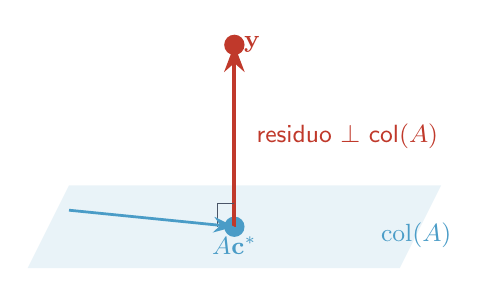
\begin{tikzpicture}[scale=1.05]
        \fill[accentblue!12](-2,-0.6)--(2.5,-0.6)--(3,0.4)--(-1.5,0.4)--cycle;
        \node[font=\small,color=accentblue]at(2.7,-0.2){$\mathrm{col}(A)$};
        \fill[accentred](0.5,2.1)circle(3.5pt)
          node[right,font=\small]{$\mathbf{y}$};
        \fill[accentblue](0.5,-0.1)circle(3.5pt)
          node[below,font=\small]{$A\mathbf{c}^*$};
        \draw[accentred,-{Stealth},line width=1.5pt](0.5,-0.1)--(0.5,2.1);
        \node[right,font=\small,color=accentred]at(0.65,1.0){residuo $\perp$ col$(A)$};
        \draw[textmid,thin](0.5,0.18)--(0.3,0.18)--(0.3,-0.1);
        \draw[accentblue,-{Stealth},line width=1pt](-1.5,0.1)--(0.5,-0.1);
      \end{tikzpicture}
      \end{center}

      \begin{lstlisting}
import numpy as np
# A: matriz de colocacion
# y: datos
c, res, rank, sv = np.linalg.lstsq(
        A, y, rcond=None)
# equivalente: resolver A^T A c = A^T y
      \end{lstlisting}
  \end{columns}
\end{frame}


% ══════════════════════════════════════════════════════════════════════════════
\sectionslide{4}{PCA}{La base \'optima emerge de los datos}

\begin{frame}[fragile]{PCA: el mismo problema, base adaptativa}
  \begin{columns}[T]
    \column{0.50\textwidth}
      Datos: $X\in\R^{N\times d}$ ($N$ observaciones, $d$ variables).

      \textbf{Mismo problema que LS}: aproximar $X$ con un subespacio de dimensi\'on $k<d$.

      \vspace{0.2cm}
      \fmbox[accentblue]{\min_{\mathrm{rango}(B)\le k}\;\norm{X - B}_F^2}

      \vspace{0.1cm}
      Diferencia clave: la \textbf{base} $\{\phi_i\}$ no es fija, se optimiza.


    \column{0.46\textwidth}
      \begin{center}
      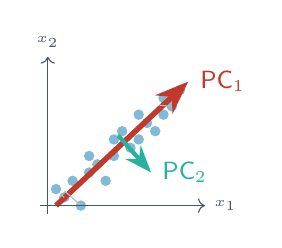
\begin{tikzpicture}[scale=1.05]
        % Nube de puntos
        \foreach \x/\y in {
          0.2/0.1, 0.5/0.4, 0.8/0.6, 1.1/0.8, 1.4/1.1,
          0.3/0.3, 0.6/0.5, 0.9/0.9, 1.2/1.0, 1.5/1.2,
          0.4/0.0, 0.7/0.3, 1.0/0.7, 1.3/0.9, 1.6/1.4,
          0.1/0.2, 0.8/0.8, 1.1/1.1, 0.5/0.6, 1.4/1.3}{
          \fill[accentblue!70](\x,\y)circle(1.8pt);}
        % PC1
        \draw[accentred,-{Stealth},line width=2pt](0.1,0.0)--(1.7,1.5)
          node[right,font=\small,color=accentred]{PC$_1$};
        % PC2
        \draw[accentteal,-{Stealth},line width=1.5pt](0.85,0.85)--+(0.4,-0.45)
          node[right,font=\small,color=accentteal]{PC$_2$};
        % Proyecciones
        \foreach \x/\y/\px/\py in {
          0.2/0.1/0.15/0.135, 1.5/1.2/1.35/1.215, 0.4/0.0/0.2/0.18}{
          \draw[textmid!40,thin](\x,\y)--(\px,\py);}
        \draw[->,thin,textmid](-0.1,0)--(1.9,0)node[right]{\tiny$x_1$};
        \draw[->,thin,textmid](0,-0.1)--(0,1.8)node[above]{\tiny$x_2$};
      \end{tikzpicture}
      \end{center}

      \begin{lstlisting}
from sklearn.decomposition import PCA
pca = PCA(n_components=2)
pca.fit(X)
      \end{lstlisting}
  \end{columns}
\end{frame}

%\begin{frame}[fragile]{La SVD: c\'omo se computa PCA}
%  Centrar los datos: $\tilde{X} = X - \bar{X}$.
%
%  \fmbox[accentblue]{\tilde{X} = U\Sigma V^T, \quad U\in\R^{N\times d},\quad \Sigma=\mathrm{diag}(\sigma_1\ge\cdots\ge\sigma_d\ge0),\quad V\in\R^{d\times d}}
%
%  \begin{columns}[T]
%    \column{0.48\textwidth}
%      \begin{itemize}
%        \item Columnas de $V$: \textbf{componentes principales} (la base \'optima)
%        \item $\sigma_i^2/(N-1)$: varianza explicada por PC$_i$
%        \item Proyecci\'on sobre $k$ componentes: $Z = \tilde{X}V_k$
%        \item Reconstrucci\'on: $\hat{X} = ZV_k^T + \bar{X}$
%      \end{itemize}
%
%
%    \column{0.48\textwidth}
%      {\small \begin{exampleblock}{Conexi\'on con $A^TA$}
%        $\tilde{X}^T\tilde{X} = V\Sigma^2 V^T$ es la \textbf{matriz de covarianza}.\\
%        Las columnas de $V$ son sus \textbf{autovectores}.
%      \end{exampleblock}}
%      
%      \vspace{0.2cm}
%\begin{lstlisting}
%X_c = X - X.mean(axis=0)
%U, s, Vt = np.linalg.svd(X_c,
%full_matrices=False)
%# componentes principales
%V = Vt.T
%\end{lstlisting}
%      
%  \end{columns}
%\end{frame}

\begin{frame}[fragile]{Teorema de Eckart--Young: PCA es LS en matrices}
  \vspace{0.1cm}
  \begin{center}
  \tikz\node[draw=accentgold,fill=boxgold,rounded corners=4pt,
             inner sep=10pt,line width=1.5pt,text width=12cm,align=center]{%
    \textbf{\color{accentgold}Teorema de Eckart--Young (1936)}\\[6pt]
    La mejor aproximaci\'on de rango $k$ de $\tilde{X}$ en norma de Frobenius es:\\[6pt]
    $B = U_k\Sigma_k V_k^T = \sum_{i=1}^k \sigma_i\,\mathbf{u}_i\mathbf{v}_i^T$\\[6pt]
    donde $U_k,\Sigma_k,V_k$ son las primeras $k$ columnas/valores singulares de la SVD.};
  \end{center}

  \vspace{0.2cm}
      \textbf{Es el mismo problema que LS}, pero en espacio de matrices:
      \[\min_{\mathrm{rango}(B)\le k}\;\norm{\tilde{X}-B}_F^2 = \sum_{i=k+1}^d\sigma_i^2\]

\end{frame}

% ══════════════════════════════════════════════════════════════════════════════
\begin{frame}{Una sola idea}
  \begin{center}
  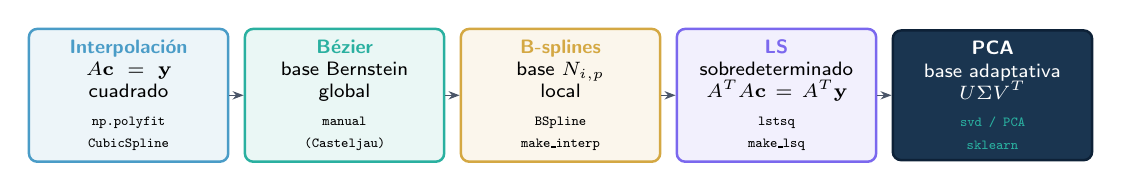
\begin{tikzpicture}[node distance=0.3cm and 0.18cm,
      arr/.style={-{Stealth[length=4pt]},textmid,thin},
      arr/.style={-{Stealth[length=4pt]},textmid,thin}]
    \node[draw=accentblue,fill=accentblue!10,rounded corners=3pt,inner sep=4pt,
          text width=2.25cm,align=center,font=\scriptsize,line width=0.9pt](a1){
      \textbf{\color{accentblue}Interpolaci\'on}\\
      $A\vc=\vy$\\cuadrado\\[2pt]
      \texttt{\tiny np.polyfit}\\
      \texttt{\tiny CubicSpline}};
    \node[draw=accentteal,fill=accentteal!10,rounded corners=3pt,inner sep=4pt,
          text width=2.25cm,align=center,font=\scriptsize,line width=0.9pt,right=of a1](a2){
      \textbf{\color{accentteal}B\'ezier}\\
      base Bernstein\\global\\[2pt]
      \texttt{\tiny manual}\\
      \texttt{\tiny (Casteljau)}};
    \node[draw=accentgold,fill=accentgold!10,rounded corners=3pt,inner sep=4pt,
          text width=2.25cm,align=center,font=\scriptsize,line width=0.9pt,right=of a2](a3){
      \textbf{\color{accentgold}B-splines}\\
      base $N_{i,p}$\\local\\[2pt]
      \texttt{\tiny BSpline}\\
      \texttt{\tiny make\_interp}};
    \node[draw=accentpurple,fill=accentpurple!10,rounded corners=3pt,inner sep=4pt,
          text width=2.25cm,align=center,font=\scriptsize,line width=0.9pt,right=of a3](a4){
      \textbf{\color{accentpurple}LS}\\
      sobredeterminado\\$A^TA\vc=A^T\vy$\\[2pt]
      \texttt{\tiny lstsq}\\
      \texttt{\tiny make\_lsq}};
    \node[draw=darkbg,fill=midbg,rounded corners=3pt,inner sep=4pt,
          text width=2.25cm,align=center,font=\scriptsize,line width=0.9pt,right=of a4](a6){
      \textbf{\color{white}PCA}\\
      \color{white}base adaptativa\\
      \color{white}$U\Sigma V^T$\\[2pt]
      \texttt{\tiny\color{accentteal}svd / PCA}\\
      \texttt{\tiny\color{accentteal}sklearn}};
    \draw[-{Stealth[length=4pt]},textmid,thin](a1)--(a2);
    \draw[-{Stealth[length=4pt]},textmid,thin](a2)--(a3);
    \draw[-{Stealth[length=4pt]},textmid,thin](a3)--(a4);
    \draw[-{Stealth[length=4pt]},textmid,thin](a4)--(a6);
  \end{tikzpicture}
  \end{center}
  
  \vspace{1cm}
  \fontsize{16}{18}\selectfont
  Todos los m\'etodos son $\displaystyle f = \sum_i c_i\phi_i$.\\[8pt]
  Lo que cambia es c\'omo \textbf{eliges la base}

\end{frame}

\end{document}
